\documentclass{beamer}
%%%%%% UNOFFICIAL ICL BEAMER TEMPLATE V.0.1 %%%%%%
% This is a basic LaTeX Beamer template that I customised to have the logo of ICL and a background picture. Mind that this is NOT an official ICL template but it may still be useful for informal presentations.
% The official ICL graphical identity resources can be found here: http://www3.imperial.ac.uk/graphicidentity
% Please drop me an e-mail or comment via Twitter @AJunyentFerre if you found this was useful or have any suggestion to improve it.
%%%%%%

\usepackage[english]{babel}

%%%%%% THE FOLLOWING FILE CONTAINS THE STYLE DEFINITIONS %%%%%%
\usepackage[utf8]{inputenc}
\usepackage{graphicx} % Allows including images
\usepackage{booktabs} % Allows the use of \toprule, \midrule and \bottomrule in tables

\definecolor{gris}{rgb}{0.92,0.92,0.92}
\definecolor{blau-upc}{rgb}{.192,.365,.506}

\setbeamercolor{titlelike}{fg=blau-upc}
% \setbeamercolor{barra}{bg=white,fg=white}
\setbeamercolor{capcalera}{bg=blau-upc,fg=white}
\setbeamercolor{section in toc}{fg=blau-upc}
\setbeamertemplate{sections/subsections in toc}[circle]
\setbeamertemplate{itemize items}[circle]
\setbeamercolor{item}{fg=blau-upc}
\setbeamertemplate{blocks}[rounded][shadow=true]
\setbeamercolor*{block body}{bg=gris}
\setbeamerfont{block body}{size=\footnotesize}
\setbeamercolor*{block title}{parent=structure,bg=blau-upc,fg=white}

\setbeamersize{text margin left=12mm,text margin right=12mm}
\setbeamertemplate{navigation symbols}{}

\defbeamertemplate*{headline}{infolines theme}
{	
	\begin{beamercolorbox}[wd=\paperwidth,ht=9.5mm,right]{white}%
		
\includegraphics[height=7mm]{../figures/imperial.png}\hspace*{3mm}
		\vskip0.2ex
	\end{beamercolorbox}
}

\setbeamertemplate{footline}
{
	\hbox{
	\begin{beamercolorbox}[wd=0.1\paperwidth,ht=10mm,left]{}
	\end{beamercolorbox}
	\begin{beamercolorbox}[wd=0.8\paperwidth,ht=3ex,center]{}
		\hspace*{4ex}\insertsection\vskip 4ex
	\end{beamercolorbox}
	\begin{beamercolorbox}[wd=0.1\paperwidth,ht=3ex,right]{}
		\insertpagenumber\hspace*{6ex}\vskip 4ex
	\end{beamercolorbox}
	}
}

\setbeamertemplate{title page}
{
	\vbox{}
	\vfill
	\begin{centering}
		{\usebeamerfont{title}\usebeamercolor[fg]{title}\inserttitle}
		\vskip0.2em
		{\usebeamerfont{subtitle}\usebeamercolor[fg]{subtitle}\insertsubtitle}
		\vskip2em\par
		\small\insertauthor\par
		\vskip0.7em\par
		\tiny\insertdate\vskip1em\par
	\end{centering}
	\vfill
}

%%%%%%

%%%%%% TITLE, AUTHOR, DATE DEFINITIONS %%%%%%
\title{Tackling Crohn's Disease using Deep Learning}
\author{Feifan Fan}
\date{\today}
%%%%%%

\begin{document}

{
	\usebackgroundtemplate{\put(-50,-340){
\includegraphics[width=10cm]{../figures/imperialback.png}}} 
	\frame{\titlepage}
}

\begin{frame}
	\frametitle{Outline} % Table of contents slide, comment this block out to remove it
	\tableofcontents % Throughout your presentation, if you choose to use \section{} and \subsection{} commands, these will automatically be printed on this slide as an overview of your presentation
\end{frame}
	
	%----------------------------------------------------------------------------------------
	%	PRESENTATION SLIDES
	%----------------------------------------------------------------------------------------
	
	%------------------------------------------------
\section{Introduction} % Sections can be created in order to organize your presentation into discrete blocks, all sections and subsections are automatically printed in the table of contents as an overview of the talk
%------------------------------------------------
\begin{frame}
	\frametitle{Overview of this Project}
	%Elaborate the purpose of your research
	%For example:
	\begin{figure}[hp]
		\centering
		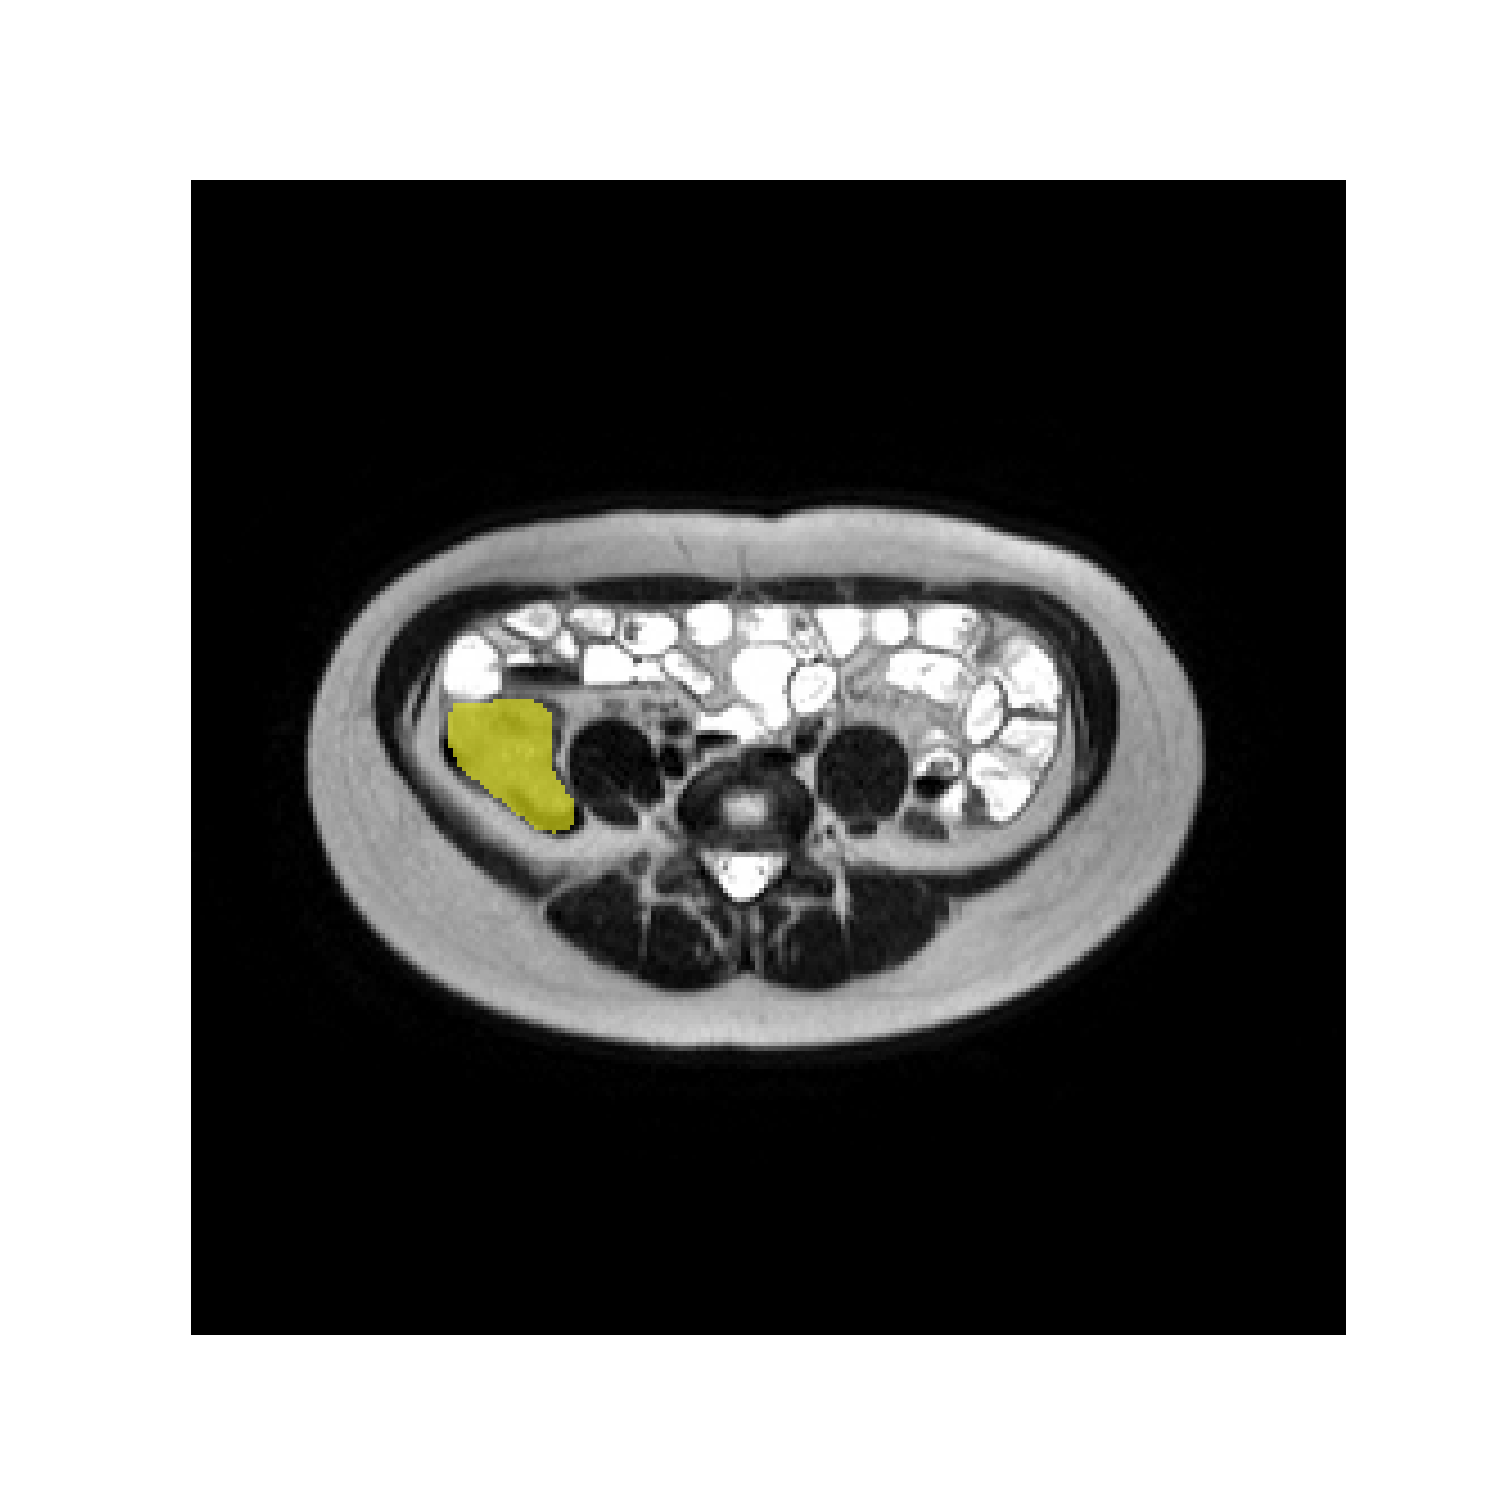
\includegraphics[width=0.5\textwidth]{../figures/seg_medsam.png}
	\end{figure}
\end{frame}

\begin{frame}
\frametitle{Crohn's Disease}

\begin{columns}[c] % The "c" option specifies centered vertical alignment while the "t" option is used for top vertical alignment

	\column{.48\textwidth} % Left column and width
	\begin{itemize}
		\item Crohn's disease is a chronic, incurable type of Inflammatory Bowel Disease (IBD).
		\item It affects over half a million individuals in the UK and can cause serious complications.
		\item Symptoms of Crohn's disease are diverse and can include abdominal pain, diarrhea, fatigue, and weight loss.
		\end{itemize}
	
	\column{.48\textwidth} % Right column and width
	\begin{figure}[htp]
		\centering
		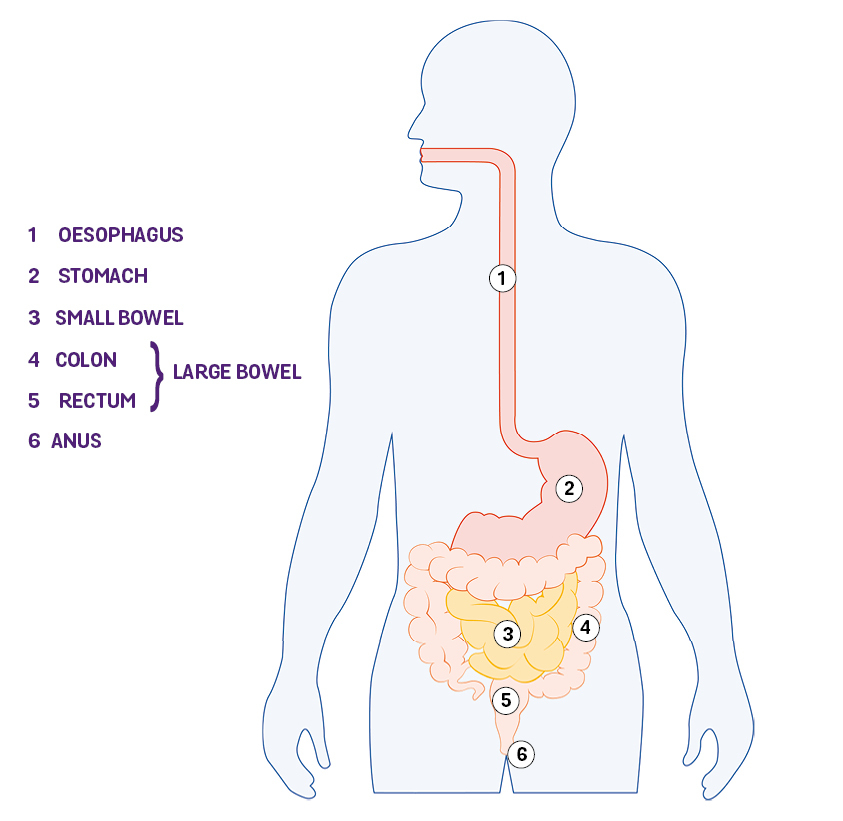
\includegraphics[width=\textwidth]{../figures/digestion-graphic.jpg}
		\caption{The gastrointestinal tract of a Human}
		\label{fig:gi-tract}
	\end{figure}
	
	\end{columns}
\end{frame}

\begin{frame}
	\frametitle{Terminal Ileum}
	\begin{columns}[c] % The "c" option specifies centered vertical alignment while the "t" option is used for top vertical alignment
		\column{.48\textwidth} % Left column and width
		\begin{itemize}
			
			\item Examination of the terminal ileum can significantly improve patient outcomes.

			\item Related work found a strong correlation between the performance of the automated detection of Crohn's disease and the degree of localisation in the training data. 
			\end{itemize}
		
		\column{.48\textwidth} % Right column and width
		\begin{figure}[htp]
			\centering
			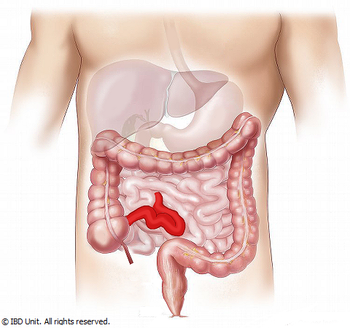
\includegraphics[width=\textwidth]{../figures/crohn's_ileitis-350x328.png}
			\caption{Terminal Ileum}
			\label{fig:terminal-ileum}
		\end{figure}
		
		\end{columns}
\end{frame}

\begin{frame}
	\frametitle{T2-weighted MR Images}
	\begin{columns}[c] % The "c" option specifies centered vertical alignment while the "t" option is used for top vertical alignment
		\column{.48\textwidth} % Left column and width
		\begin{figure}[ht]
			\centering
			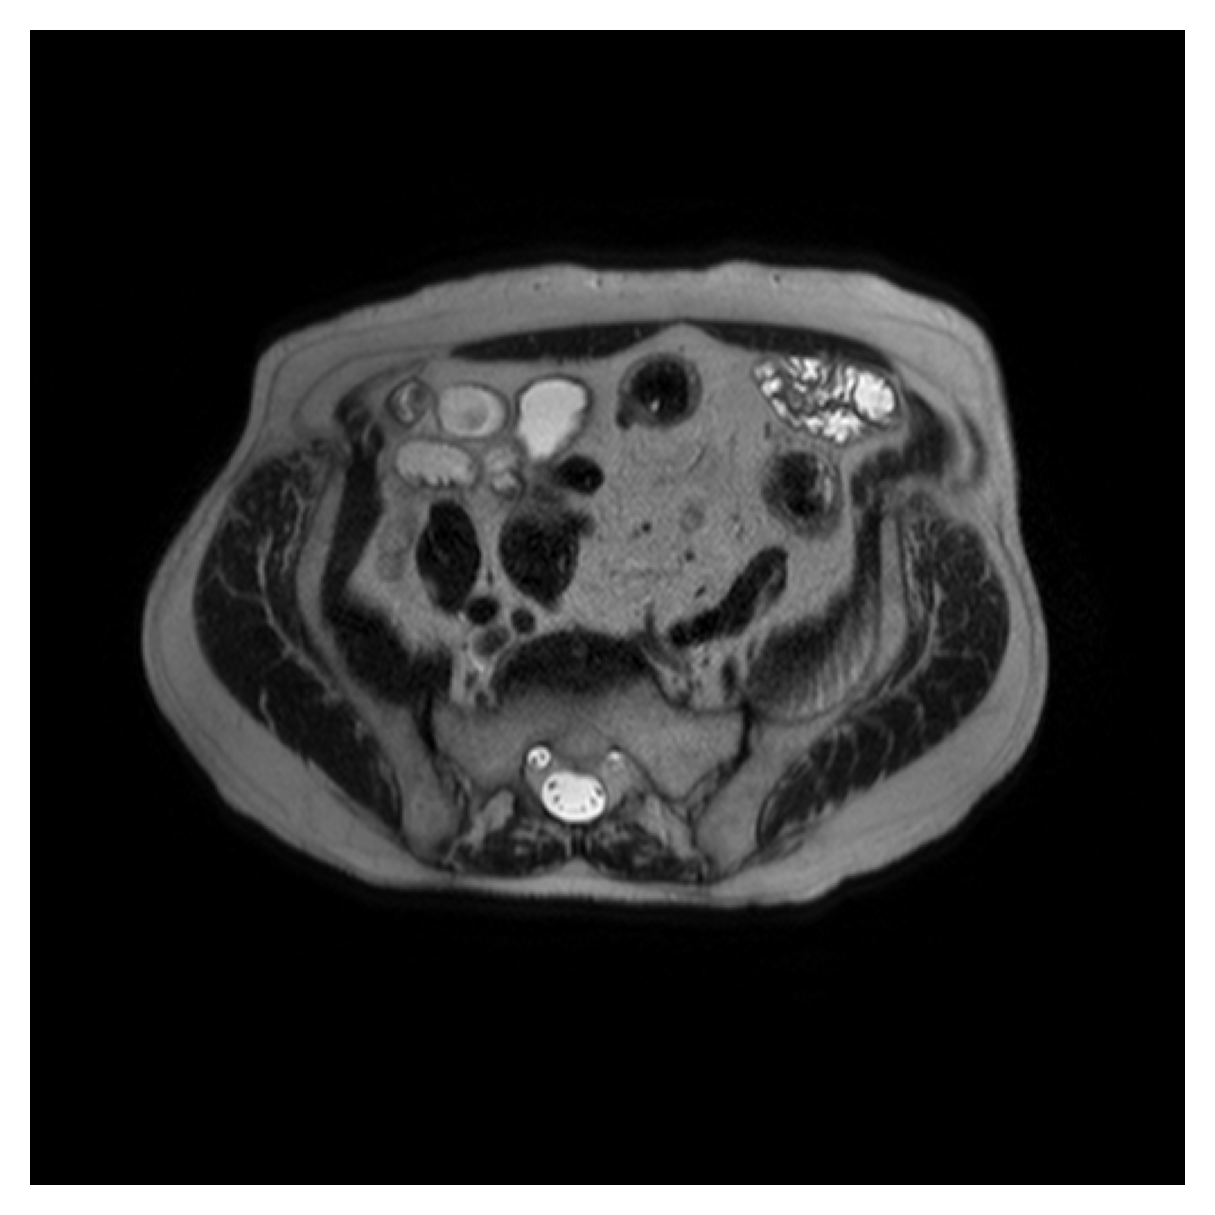
\includegraphics[width=0.8\textwidth]{../figures/axial.png}
			\caption{Axial T2 MR Image}
			\label{fig:axial-t2}
		\end{figure}
		
		\column{.48\textwidth} % Right column and width
		\begin{figure}[ht]
			\centering
			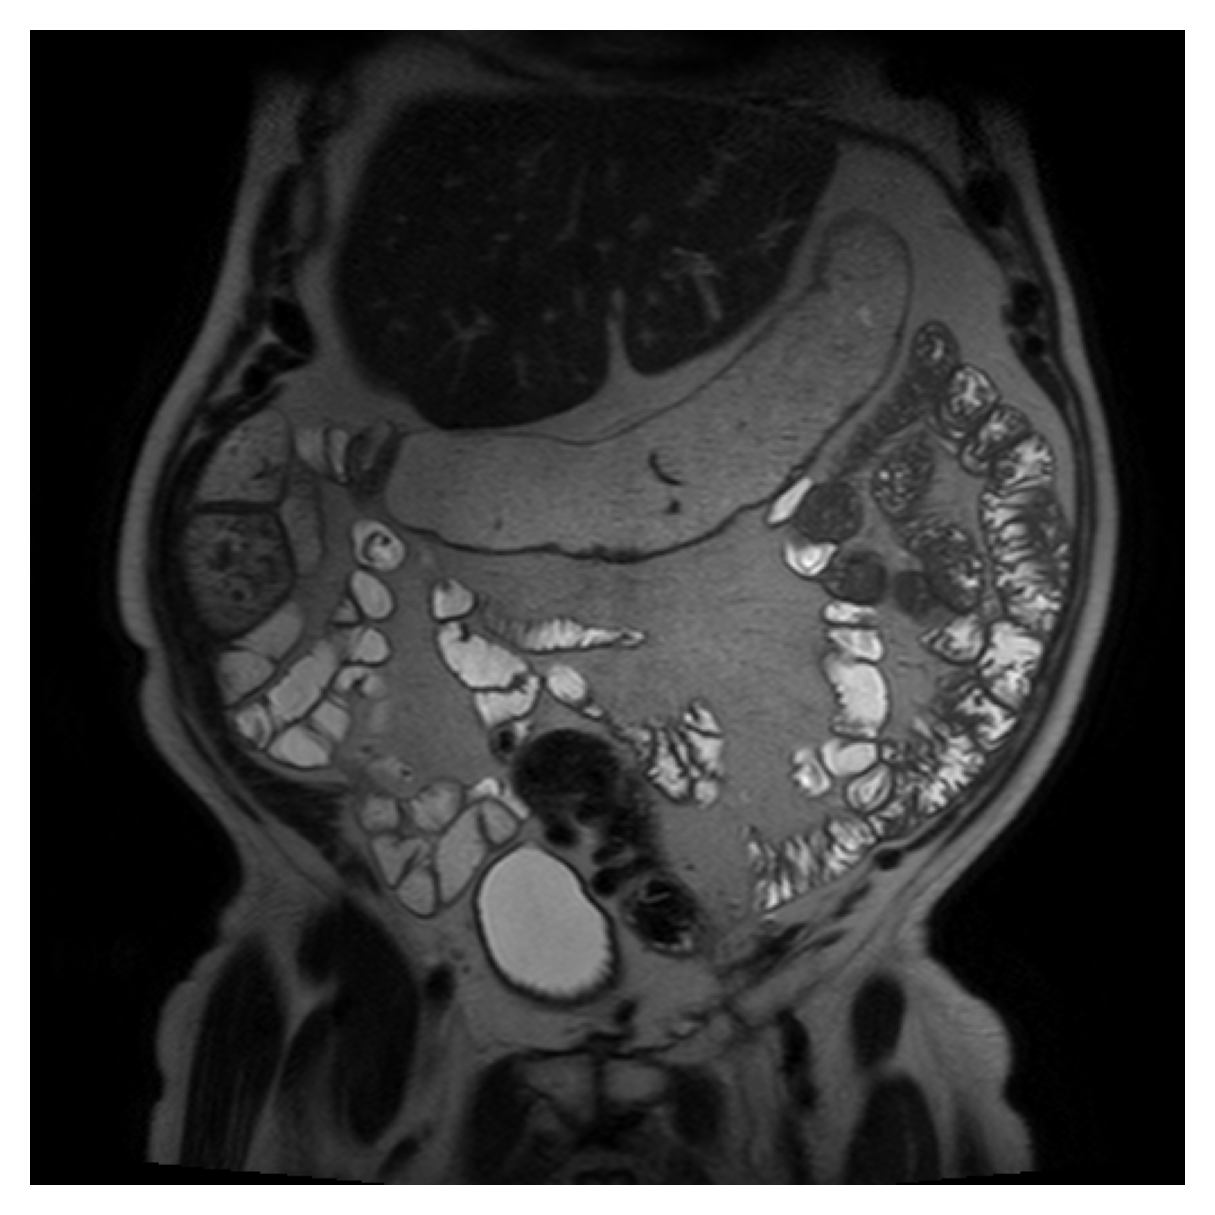
\includegraphics[width=0.8\textwidth]{../figures/coronal.png}
			\caption{Coronal T2 MR Image}
			\label{fig:coronal-t2}
		\end{figure}
		
		\end{columns}
\end{frame}

% ------------------------------------------------

\begin{frame}
\frametitle{Machine Learning Challenges}
\begin{block}{Limited Dataset}
We had only 233 cases for both modalities (Axial and Coronal T2 images) collected by St Mark's Hospital. Data scarcity limits the potential to train a high-performing and generalized model.
\end{block}

\begin{block}{Lack of Gold-Standard Labels}
We had only less than 40 gold-standard segmentations for each modality. Generating gold-standard segmentation is often time-consuming and requires expert knowledge which further adds to this challenge.
\end{block}

\begin{block}{Utilisation of Unlabelled Data}
Another challenge lies in finding an effective way to utilise the unlabelled data in the training process, which also contributes to creating a more comprehensive and robust model.
\end{block}
\end{frame}

% ------------------------------------------------
\section{Methodology}
% ------------------------------------------------

\begin{frame}
	\frametitle{Overview of the Methodology}
	Our methodology involves a two-phased training algorithm to effectively utilise the available data and maintain segmentation precision. 
\begin{itemize}
	\item \textbf{Proxy Model Training:} The initial phase involves generating "weak labels" for the unannotated data using a fine-tuned MedSAM model. A proxy model is then trained on these weak labels using the nnU-Net architecture.
	\item \textbf{Target Model Training:} The second phase leverages the proxy model, further training it on 80\% of fully annotated data to generate the final target model.
\end{itemize}
This approach aims to maximise data utilisation and maintain high precision in the terminal ileum segmentation. The effectiveness of the model is assessed by the Dice similarity coefficient on the remaining 20\% of the fully annotated data.
\end{frame}
\begin{frame}
\frametitle{Table}
\begin{table}
\begin{tabular}{l l l}
\toprule
\textbf{Treatments} & \textbf{Response 1} & \textbf{Response 2}\\
\midrule
Treatment 1 & 0.0003262 & 0.562 \\
Treatment 2 & 0.0015681 & 0.910 \\
Treatment 3 & 0.0009271 & 0.296 \\
\bottomrule
\end{tabular}
\caption{Table caption}
\end{table}
\end{frame}
	
% ------------------------------------------------

\begin{frame}
\frametitle{Theorem}
\begin{theorem}[Mass--energy equivalence]
$E = mc^2$
\end{theorem}
\end{frame}

% ------------------------------------------------
	
\begin{frame}[fragile] % Need to use the fragile option when verbatim is used in the slide
\frametitle{Verbatim}
\begin{example}[Theorem Slide Code]
\begin{verbatim}
\begin{frame}
\frametitle{Theorem}
\begin{theorem}[Mass--energy equivalence]
$E = mc^2$
\end{theorem}
\end{frame}\end{verbatim}
\end{example}
\end{frame}

% ------------------------------------------------
	
\begin{frame}
\frametitle{Figure}
Uncomment the code on this slide to include your own image from the same directory as the template .TeX file.
%\begin{figure}
%\includegraphics[width=0.8\linewidth]{test}
%\end{figure}
\end{frame}

% ------------------------------------------------

\begin{frame}[fragile] % Need to use the fragile option when verbatim is used in the slide
\frametitle{Citation}
An example of the \verb|\cite| command to cite within the presentation:\\~

This statement requires citation \cite{p1}.
\end{frame}

% ------------------------------------------------
	
\begin{frame}
\frametitle{References}
\footnotesize{
\begin{thebibliography}{99} % Beamer does not support BibTeX so references must be inserted manually as below
\bibitem[Smith, 2012]{p1} John Smith (2012)
\newblock Title of the publication
\newblock \emph{Journal Name} 12(3), 45 -- 678.
\end{thebibliography}
}
\end{frame}

% ------------------------------------------------

\begin{frame}
\Huge{\centerline{\LARGE \usebeamercolor[fg]{title} Thank you for your attention}}
\end{frame}


\end{document}